% 2. Fragen zur Vorbereitung

\chapter{Fragen zur Vorbereitung}
\label{chap:fvz}

% Text

% Input der Teilaufgaben je nach Produktion der Nebendateien ohne Ordner
% Teilaufgabe 1

\section{Rauschquellen}

\paragraph*{Quantenrauschen}
Aufgrund der Quantisierung des Lichtes (in Photonen) ist es aus statistischen Gründen unmöglich, dass die Intensität der Lichtes absolut konstant ist. Es gilt folgender Zusammenhang für das mittlere Quadrat des Rauschstromes:
\begin{gather}
    i^2_Q = 2ei_{Ph}\Delta \nu = \frac{2e^2\beta_D}{hc}\lambda P \Delta \nu
\end{gather}
wobei\\
\begin{tabular}{rl}
    $e$: & Elementarladung \\
    $i_{Ph}$: & Photonenstrom des Detektors\\
    $\Delta \nu$: & Detektionsbandbreite\\
    $\beta_D$: & Quantenausbeute (Nachweiswahrscheinlichkeit) des Detektors\\
    $\lambda$: & Wellenlänge\\
    $P$: & Lichtleistung\\
    $h$: & Planksches Wirkungsquantum\\
    $c$: & Lichtgeschwindigkeit
\end{tabular}\\
Es ist deutlich zu sehen, dass das Quantenrauschen mit der Quantenausbeute, der Wellenlänge, der Lichtleistung und der Detektionsbandbreite ansteigt.

\paragraph*{Thermisches Rauschen der Photodiode}
Dieses Rauschen ensteht durch die thermische Bewegung der Elektronen in der Photodiode. Die thermische Rauschleistung ergibt sich folgendermaßen:
\begin{gather}
    P_T = 4 k_B T \Delta \nu
\end{gather}
wobei $k_B$ der Boltzmannfaktor, $T$ die absolute Temperatur ist und $\Delta \nu$ die Detektionsbandbreite. Somit ist auch klar ersichtlich, dass dieses Rauschen mit der Temperatur und Detektionsbandbreite zunimmt.


\paragraph*{Technisches Laserrauschen}
Dieses Rauschen tritt Aufgrund der Technischen eigenheiten des Lasers auf. Beispielsweise kann dieses Rauschen durch Schwingungen der Laserspiegel zueinander oder Instabilitäten in der Gasentladung, bei Gaslasern, verursacht werden. Eine Besonderheit dieses Rauschens ist es, dass es nicht weiß ist, sondern es vor allem bei niedrigen Frequenzen auftritt. Oberhalb einiger MHz ist es dann vernachlässigbar. 

% Teilaufgabe X

\section{Vergleich thermisches Rauschen und Quantenrauschen}
\label{sec:rauschen}

Im Folgenden soll die Leistung (in dBm) de thermischen Rauschens und des Quantenrauschens für folgenden Fall berechnet werden:

$P = 0,1$ mW, $T = 293$ K, $R = 50\, \Omega$, $\beta_D = 0,3$ und $\Delta \nu = 10$ kHz.

Für die Leisungsschwankung, welch durch Quantenrauschen verursacht wird, gilt:
\begin{align}
    \Delta P_\mathrm{Q} &= i^2_\mathrm{Q} \cdot R = \frac{2e^2\beta_\mathrm{D}}{hc}\lambda P \Delta \nu \cdot R \\
    \Delta P_\mathrm{Q} &= \frac{2e^2 \cdot 0,3}{hc} \cdot (632,8 \cdot 10^{-9}) \, \mathrm{m} \cdot (0,1 \cdot 10^{-3})\, \mathrm{W} \cdot (10 \cdot 10^3) \, \mathrm{Hz} \cdot 50 \, \Omega \\
    \Delta P_\mathrm{Q} &= 2,45 \cdot 10^{-15}\,\mathrm{mW} \qquad \Rightarrow \quad \Delta P_\mathrm{Q}^* = -146 \, \mathrm{dBm}
\end{align}

Für das thermische Rauschen gilt:
\begin{gather}
    P_\mathrm{T} = 4 \cdot k_\mathrm{B} \cdot 293\,\text{K} \cdot 10\,\text{kHz} = 1,62 \cdot 10^{-13}\, \text{mW} \qquad \Rightarrow \quad P_\mathrm{T}^* = -128 \, \text{dBm}
\end{gather}

Es ist zu erkennen, dass das Quantenrauschen gegenüber dem thermischen Rauschen zu vernachlässigen ist.
Somit reicht es die Verstärkung und die Verringerung von 6\,dbm \cite{anleitung} auf das thermische Rauschen anzuwenden, um den Rauschpegel zu erhalten:
\begin{gather}
    P_\mathrm{R,Theo}^* = -128 \, \text{dBm} + 55\, \text{dBm} - 6 \, \text{dBm}= -79 \, \text{dBm}
\end{gather}
% Teilaufgabe 3

\section{Dunkelfeldmikroskop in Transmission}
\label{sec:mikroskop}

\subsection{Aufbau und Funktionsweise}
\label{sub:aufbau}

\begin{center}
    \captionsetup{type = figure}
    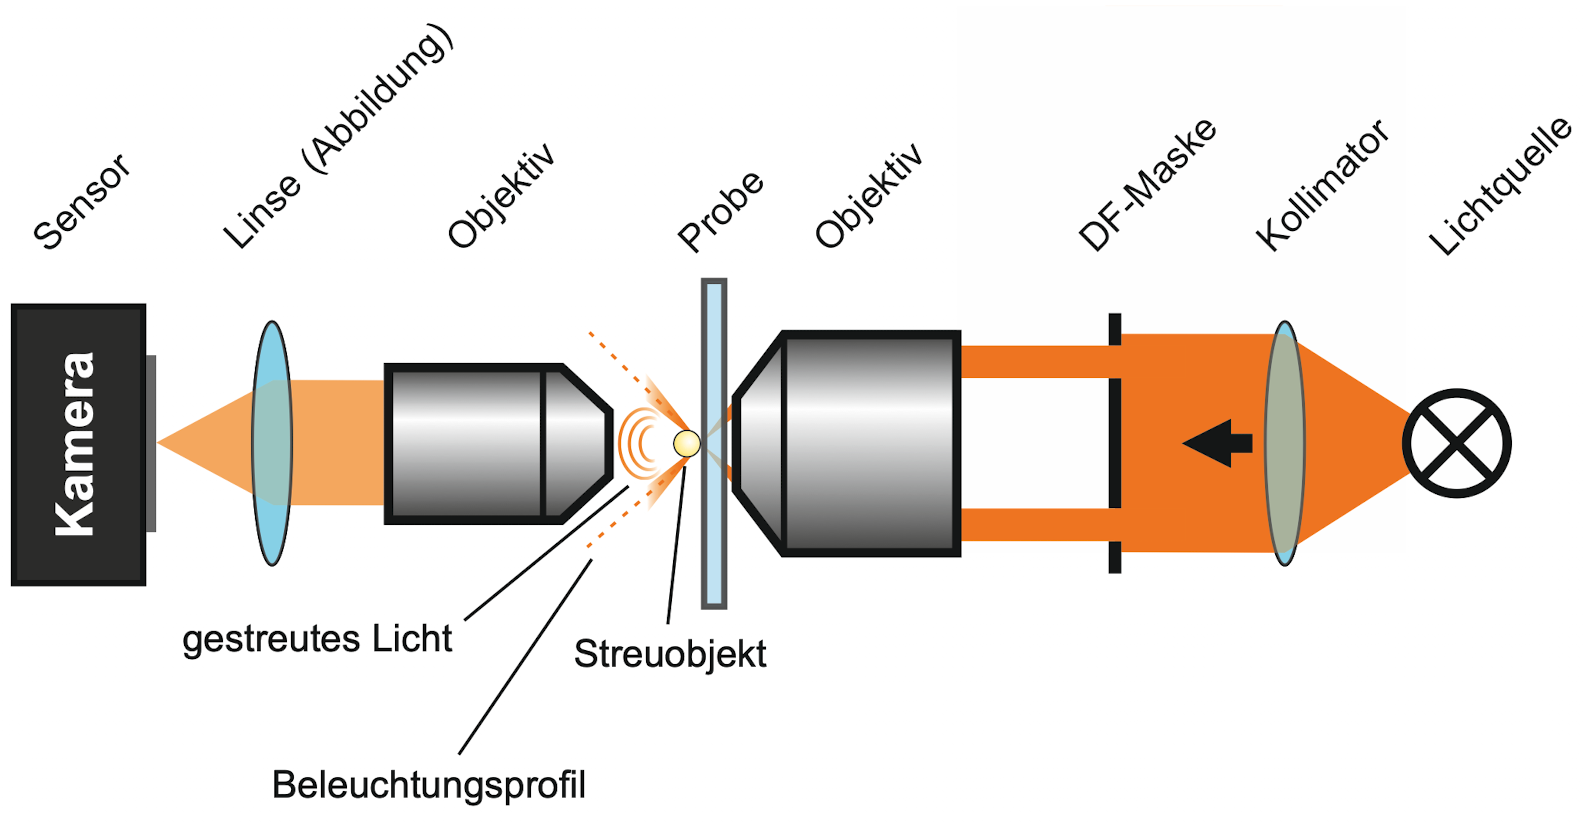
\includegraphics[width = 0.9\textwidth]{Bilder/Aufbau_Dunkelfeld.png}
    \captionof{figure}{Einfacher Aufbau eines Dunkelfeldmikroskops in Transmission. Eine breitbandige Lichtquelle wird mittels einer Optik kollimiert. Eine Maske (DF-Maske) schneidet einen Ring in das Strahlprofil. Der so geformte Strahl wird mittels Objektiv auf die Probe fokussiert. Ein weiteres Objektiv sammelt das von der Probenoberfläche bzw. dem Objekt gestreute Licht auf, wodurch kein direktes Licht der Beleuchtung eingesammelt wird. Das gestreute Licht wird über eine Linse auf den Kamerasensor abgebildet. \cite{Anleitung}}
    \label{fig:aufbau}
\end{center}

Die Dunkelfeldmikroskopie ist eine hintergrundfreie Methode, was bedeutet, dass kein Hintergrundsignal detektiert wird, sondern nur Informationen von dem untersuchten Objekten. In Abb. \ref{fig:aufbau} ist der schematische Aufbau des Dunkelfeldmikroskops in Transimission abgebildet. Auf der rechten Seite steht die Lichtquelle, die mittels einer Linse kollimiert wird. Dahinter befindet sich eine inverse Lochblende (DF-Maske), die lediglich die Ränder des Lichtkegels transmittiert. Mit einem Objektiv relativ hoher numerischer Apertur wird die Probe beleuchtet, wobei auf der anderen Seite der Probe befindet sich ein Objektiv mit geringerer numerischer Apertur. Durch diese besondere Beleuchtung kann kein direktes Erregerlicht in dieses Objektiv fallen, wodurch die Abbildung der Probenoberfläche auf der Kamera dunkel erscheint. Befindet sich jedoch ein Streukörper, zum Beispiel ein Nanopartikel, auf der Probenoberfläche so wird das Erregerlicht daran gestreut, was widerum vom Objektiv aufgesammelt und detektiert werden kann. \cite{Anleitung}

\subsection{Messung von plasmonischen Eigenschaften}
\label{sub:messungEigenschaften}

Das Prinzip der Dunkelfeldmikroskopie beruht darauf, dass Objekte Licht nicht nur absorbieren, sondern auch immer einen Teil des Lichtstrahls ablenken. Die Stärke eines Signals ist bei der Dunkelfeldmikroskopie nicht von der Größe einer Struktur abhängig, sondern davon wie stark das Licht von ihr abgelenkt wird. Eine der Ablenkungsursachen ist die als Tyndall-Effekt bezeichnete Streuung von Licht an kleinen Teilchen, welche beispielsweise auch zu beobachten ist, wenn Licht in einen dunklen Raum fällt und der Staub innerhalb des Lichtstrahls deutlich sichtbar wird. Daher können auch Partikel oder Strukturen nachgewiesen werden, die kleiner sind als die Auflösungsgrenze des jeweiligen Mikroskops. \cite{WikiDunkelfeld}

\subsection{Hintergrundkorrigiertes Dunkelfeldspektrum}
\label{sub:korrigiertesSignal}

In diesem Versuch wird zusätzlich zum hintergrundfreien Streuspektrum der Partikel auch noch das Lampenspektrum der Beleuchtungseinheit, sowie ein Spektrum ohne Beleuchtung aufgenommen. Um ein hintergrundkorrigiertes Dunkelfeldspektrum zu erhalten, wird im folgenden vom Lampenspektrum das Spektrum ohne Beleuchtung abgezogen, was im weiteren als effektives Lampenspektrum bezeichnet wird. Das effektive Lampenspektrum wird wiederum vom Streuspektrum des Partikels abgezogen, wobei hier auch das Spektrum ohne Beleuchtung abgezogen wurde. Nach dieser Argumentation wird klar, dass beide Spektren (Lampenspektrum und Streuspektrum) den gleichen Hintergrund Offset (Spektrum ohne Beleuchtung) teilen. Weshalb vorgeschlagen wird die Korrketur, um den Offset zu vernachlässigen und nur um das Lampenspektrum zu korrigieren. 
% Teilaufgabe 4

\newpage
\section{Stokes Relation}
\label{sec:stokesRelation}

\begin{align}
    t^2 + r^2 = 1 
\end{align}

Die Strokes Relation sagt aus, dass reflektierte und transmittierte Intensität zusammen die Intensität der einfallenden Welle ergeben, sofern keine Absorption durch das Material auftritt.
% Teilaufgabe X

\section{Quecksilberdampflampe als alternative Lichtquelle}

Eine Quecksilberdampflampe eignet sich nicht als Alternative für einen Laser. Wie bereits erwähnt wurde ist für FMS ein monochromatischer Laser, welcher nur in einer Mode schwingt, erforderlich. Diese Anforderungen erfüllt die Quecksilberdampflampe nicht, was zu beträchtlichen Störungen der Messung führt.

Man könnte jedoch Filter benutzen, um die gewünschte Mode herauszufiltern. Dieses Vorgehen ist jedoch mit starken Intensitätseinbusen verbunden, weshalb es auch ungeeignet ist.
% Teilaufgabe X

\section{Phasenmodulation des Laserlichtes}

Das Laserlicht wird in einem elektrooptischen Modulator phasenmoduliert. In diesem befinden sich zwei hintereinander angeordnete LiTaO$_3$-Kristalle. Diese verändern ihren Brechungsindex, für Licht einer bestimmten Polarisation, bei angelegten E-Feld. Mittels Hochfrequenzgenerator wird der Kristall nun angesteuert um die Phase des Laserstrahls zu modulieren.
% Teilaufgabe 7

\newpage
\section{Spektren der verwendeten Lampen dieses Versuches}
\label{sec:spekternLampen}

\begin{enumerate}
	\item Halogenlampe
	\begin{center}
		\captionsetup{type=figure}
		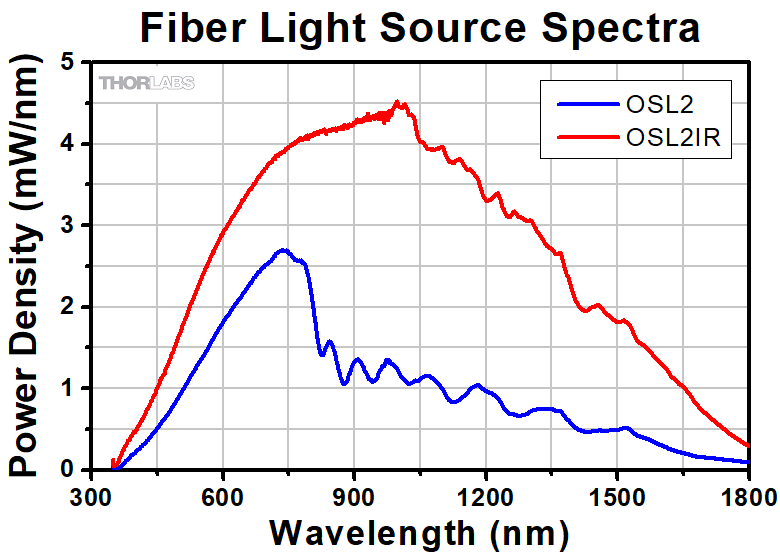
\includegraphics[width=0.75\textwidth]{Spektrum-Halogen.png}
		\captionof{figure}{Spektrum einer Halogenlampe. \cite{halogenlamp}}
		\label{fig:halogen}
	\end{center}
	\item Deuteriumlampe
	\begin{center}
		\captionsetup{type=figure}
		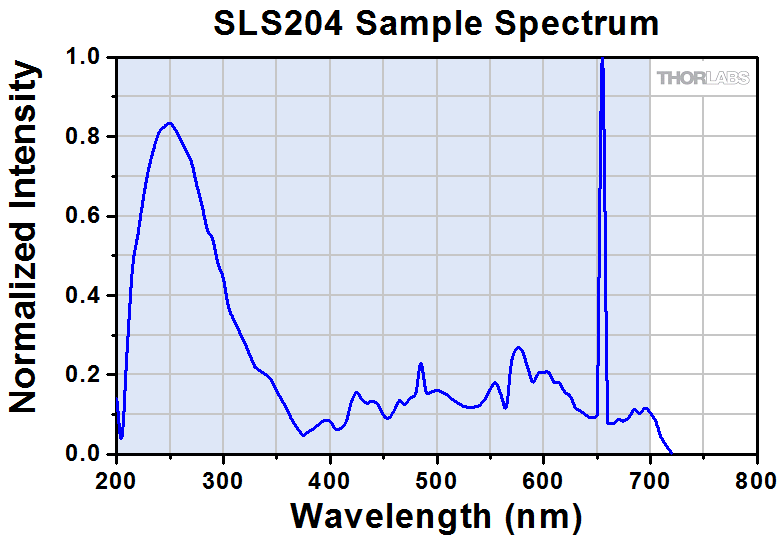
\includegraphics[width=0.75\textwidth]{Spektrum-Deuterium.png}
		\captionof{figure}{Spektrum einer Deuteriumlampe. \cite{deuteriumlamp}}
		\label{fig:deuterium}
	\end{center}
\end{enumerate}

% Teilaufgabe X

\section{Teilaufgabe X}
% Teilaufgabe X

\section{Teilaufgabe X}
% Teilaufgabe X

\section{Zusammenhang zwischen Absorptionskoeffizienten und Brechungsindex}
\label{sec:absorpBrechung}

Der Absorptionskoeffizient $\alpha$ ist proportional zum Imaginärteil des Brechungsindexes $\kappa$.  Dieser Zusammenhang kann mit einer erzwungen elektromagnetischen Schwingung der Form:
\begin{gather}
    m \derivative[2]{x}{t} + b \derivative{x}{t} + Dx = q E_0e^{i\omega t}
    \label{eq:schwingung}
\end{gather}
mit Masse $m$, Ladung $q$, Reibungskonstante $b$ und Rückstellmoment $D$ erklärt werden. Durch Lösen der Gleichung \ref{eq:schwingung} mit dem Ansatz $x=x_0e^{i\omega t}$ und Einsetzen der Lösung in die Gleichung der Polarisation $P = Nqx = \epsilon_0(\epsilon-1)E$ erhält man mit dem Brechungsindex $n$ von nichtferromagnetischen Materialien ($n = \sqrt{\epsilon}$) erhält man:
\begin{gather}
    n^2 = 1 + \frac{Nq^2}{\epsilon_0 m (\omega_0^2 - \omega^2 + i\gamma\omega)}~,
    \label{eq:brechungsindex}
\end{gather}
wobei $\gamma = b/m$ und $\omega_0^2 = D/m$ ist. Der Brechungsindex kann dann in den komplexen Brechungsindex $n(\omega)$ umgeschrieben werden:
\begin{gather}
    n = n' + i\kappa;~~~~ n',\kappa \in \mathbb{R}~.
\end{gather}
Im nächsten Schritt wird eine elektromagnetische Welle der Form:
\begin{gather}
    E = E_0 e^{i(\omega t - Kz)}~\mathrm{mit}~K = 2\pi/\lambda~,
    \label{eq:efeld}
\end{gather}
welche durch das Medium mit dem Brechungsindex $n$ in $z$-Richtung mit der Wellenzahl $K$ läuft. Im Vakuum ist dabei $K = K_0$ und in der Materie $K_\mathrm{M} = nK_0 = n'K_0 -i\kappa K_0$. Setzt man $K_\mathrm{M}$ für $K$ in Gleichung \ref{eq:efeld} ein, erhält man:
\begin{gather}
    E = E_0e^{-K_0\kappa z}e^{i(\omega t -n'K_0z)} = E_0e^{-2\pi \kappa z/ \lambda}e^{iK_0(c_0 t -n'z)}~.
    \label{eq:efeldc}
\end{gather}
Laut Beerschen Absorptionsgesetz ist der Absorptionskoeffizient $\alpha$ für den Intensitätsverlauf gegeben durch:
\begin{gather}
    I = I_0 e^{-\alpha z}~.
    \label{eq:beer}
\end{gather}
Da Intensität proportional zum Quadrat der Amplitude ist, wird Gleichung \ref{eq:efeldc} quadriert und die Exponenten mit denen der Gleichung \ref{eq:beer} verglichen. Der Vergleich ergibt dann:
\begin{gather}
    \boxed{\alpha = 4 \pi \kappa / \lambda = 2K \kappa}~,
\end{gather}
was die zuvor angesprochenen Zusammenhang ergibt. \cite{DemtroederLaser1}
% Teilaufgabe X

\section{Signal vor dem Mischer bei fester Modulationsfrequenz $\omega_\mathrm{m}$}
\label{sec:signalMischer}


% Teilaufgabe X

\section{Herleitungen}
\label{sec:herleitung}

In diesem Kapitel sollen Formel (3.6) und (3.7) aus dem Skript zu diesen Versuch hergeleitet werden. Da das Skript selbst nicht direkt auf den Ursprung der Formeln eingeht, wird diese Herleitung nur kurz mit der Literatur \citenum{FMSpectro} hergeleitet und dem Skript abgearbeitet.

Aus Literatur \citenum{FMSpectro} wird entnommen, dass folgende Relation gilt:
\begin{gather}
    \delta_\mathrm{n} = \alpha_\mathrm{n} \frac{L}{2}~.
    \label{eq:absorp}
\end{gather}
Aus dem Skript entnehmen wir von die Gleichungen (1.1) und (1.2) und setzen sie gleich, was folgende Beziehung ergibt:
\begin{gather}
    \frac{I}{I_0} = e^{-\alpha L} = 10^{-\mathrm{OD}} \Leftrightarrow \alpha = \frac{\ln 10}{L} \mathrm{OD}~.
    \label{eq:absorpkoeff}
\end{gather}
Setzt man nun nur noch Gleichung \ref{eq:absorpkoeff} in Gleichung \ref{eq:absorp} erhält man die gewünschte Beziehung:
\begin{gather}
    \boxed{\delta_\mathrm{n} = \frac{\ln 10}{2} \mathrm{OD}}~.
\end{gather}

Weiterhin wird aus der Literatur \citenum{FMSpectro} entnommen:
\begin{gather}
    \phi_\mathrm{n} = \eta_\mathrm{n} L \left( \frac{\omega_\mathrm{c} + n \omega_\mathrm{m}}{c} \right)~.
    \label{eq:phase}
\end{gather}
Zusammen mit der Überlegungen
\begin{gather}
    c = \lambda f = \lambda \frac{\omega}{2\pi} \Leftrightarrow \frac{2\pi}{\lambda} = \frac{\omega}{c}~\mathrm{mit}~\omega=\omega_\mathrm{c} + n \omega_\mathrm{m}
\end{gather}
muss dann eingesetzt in Gleichung \ref{eq:phase} gelten:
\begin{gather}
    \boxed{\phi_\mathrm{n} = \eta_\mathrm{n} L \left( \frac{2\pi}{\lambda} \right)}~,
\end{gather}
was die gesuchte Gleichung (3.7) aus dem Skript ergibt.
% Teilaufgabe X

\section{Physikalische Eigenschaft der Hyperfeinstruktur von Jod und Brom}
\label{sec:hyperfeinstruktur}

Die Hyperfeinstruktur impliziert die physikalische Eigenschaft, dass die Atomkerne ein magnetisches Moment besitzen. Dabei wird das magnetische Moment in der Quantenmechanik in der Form:
\begin{gather}
    \abs{\vect{I}} = \hbar \sqrt{I\cdot (I+1)}
\end{gather}
beschrieben. \cite{DemtroederKerne} Die Aufspaltung der Hyperfeinstruktur liefern dann zwei Beiträge:
\begin{itemize}
    \item Wechselwirkung des Kernmomentes mit dem Magnetfeld, das von Elektronen am Kernort erzeugt wird (Zeeman-Effekt des Kernmomentes mit dem atomaren Magnetfeld) \cite{DemtroederAtome}
    \item Wechselwirkung des elektronischen magnetischen Moment mit dem vom Kernmoment erzeugten Magnetfeld \cite{DemtroederAtome}
\end{itemize}


% etc.